% ---------------------------------------------------------------------------
% From classical SEM to modern structural econometrics
% ECO 629 -- Studies in Quantitative Methods (Stony Brook University)
%
% Build:
%   pdflatex sem_to_structural.tex
%   pdftoppm -r 400 -png -singlefile sem_to_structural.pdf sem_to_structural
%
% Renders on an opaque white page so the image sits correctly on a white
% card in both the light and the dark theme of the course website.
% ---------------------------------------------------------------------------
\documentclass[border=6pt,11pt]{standalone}

\usepackage[T1]{fontenc}
\usepackage[utf8]{inputenc}
\usepackage[scaled]{helvet}
\renewcommand{\familydefault}{\sfdefault}

\usepackage{xcolor}
\usepackage{tikz}
\usetikzlibrary{positioning,arrows.meta,calc}

% ---- house palette --------------------------------------------------------
\definecolor{hsPrimary}{HTML}{2E7EB8}   % borders and arrows
\definecolor{hsFill}{HTML}{EAF1F8}      % light box fill
\definecolor{hsAccent}{HTML}{E0A32E}    % accent, used sparingly
\definecolor{hsText}{HTML}{1F2937}      % body text
\definecolor{hsMuted}{HTML}{5B6B7C}     % subtitles and arrow labels

% opaque white background (not transparent)
\pagecolor{white}

\begin{document}
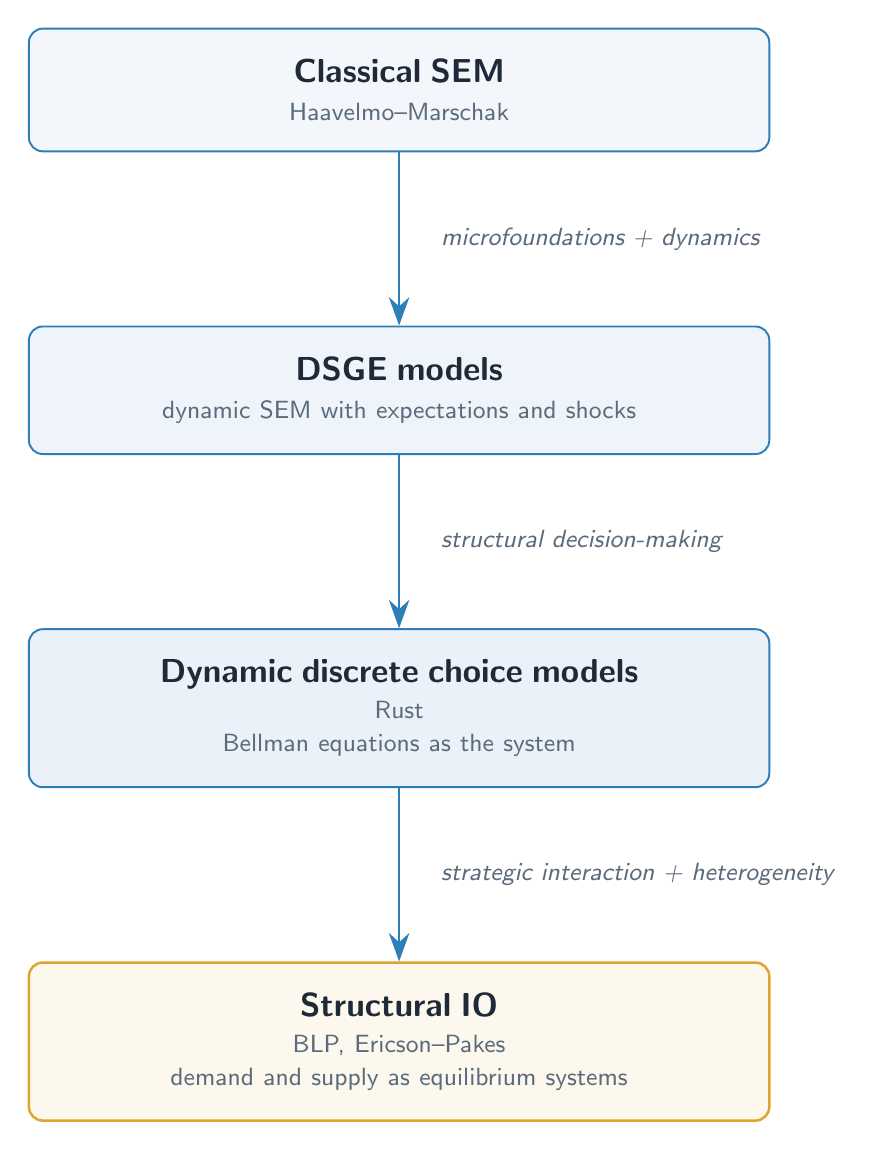
\begin{tikzpicture}[
  font=\sffamily,
  every node/.style={transform shape=false},
  box/.style={
    rectangle, rounded corners=5pt,
    draw=hsPrimary, line width=0.7pt,
    text width=8.7cm, align=center,
    inner xsep=10pt, inner ysep=11pt,
    text=hsText
  },
  % subtle progression in fill saturation: earlier = paler, later = deeper
  b1/.style={box, fill=hsFill!55!white},
  b2/.style={box, fill=hsFill!80!white},
  b3/.style={box, fill=hsFill},
  b4/.style={box, fill=hsAccent!8!white, draw=hsAccent, line width=0.9pt},
  title/.style={font=\sffamily\bfseries\large, text=hsText},
  sub/.style={font=\sffamily\small, text=hsMuted},
  flow/.style={
    -{Stealth[length=3.6mm,width=2.6mm]},
    draw=hsPrimary, line width=0.9pt
  },
  lbl/.style={
    font=\sffamily\small\itshape, text=hsMuted,
    anchor=west, xshift=4mm
  }
]

% ---- boxes ----------------------------------------------------------------
\node[b1] (sem) {
  {\bfseries\large Classical SEM}\\[2pt]
  {\small\color{hsMuted} Haavelmo--Marschak}
};

\node[b2, below=22mm of sem] (dsge) {
  {\bfseries\large DSGE models}\\[2pt]
  {\small\color{hsMuted} dynamic SEM with expectations and shocks}
};

\node[b3, below=22mm of dsge] (ddc) {
  {\bfseries\large Dynamic discrete choice models}\\[2pt]
  {\small\color{hsMuted} Rust\\ Bellman equations as the system}
};

\node[b4, below=22mm of ddc] (io) {
  {\bfseries\large Structural IO}\\[2pt]
  {\small\color{hsMuted} BLP, Ericson--Pakes\\ demand and supply as equilibrium systems}
};

% ---- arrows ---------------------------------------------------------------
\draw[flow] (sem)  -- node[lbl] {microfoundations + dynamics}      (dsge);
\draw[flow] (dsge) -- node[lbl] {structural decision-making}       (ddc);
\draw[flow] (ddc)  -- node[lbl] {strategic interaction + heterogeneity} (io);

\end{tikzpicture}
\end{document}
